User guide for version 1.0.0.

\hypertarget{installation-instructions}{%
\subsection{Installation Instructions}\label{installation-instructions}}

optoConfig-96 is available as a Python package or as standalone bundles
for Windows 10 and MacOS 10.15. Installation should not take more than 5
minutes.

\hypertarget{windows-10}{%
\subsubsection{Windows 10}\label{windows-10}}

\begin{enumerate}
\def\labelenumi{\arabic{enumi}.}
\tightlist
\item
  Download the .zip archive from the GitHub \emph{Releases} page.
\item
  Extract the archive to a location of your choice.
\item
  Run \emph{optoConfig-96.exe}. You may be asked to allow execution of
  the application.
\end{enumerate}

\hypertarget{macos}{%
\subsubsection{MacOS}\label{macos}}

\begin{enumerate}
\def\labelenumi{\arabic{enumi}.}
\tightlist
\item
  Download the .dmg disk image from the GitHub \emph{Releases} page.
\item
  Open the disk image and drag the application to the
  \emph{Applications} folder as indicated (or to another location of
  your choice).
\item
  You may be asked to allow execution of a foreign application. To do
  this, go to \emph{System Preferences \textgreater{} Security \&
  Privacy \textgreater{} General} and grant optoConfig-96 permission to
  run. Administrator rights may be required depending on your security
  settings.
\end{enumerate}

\hypertarget{as-a-python-package}{%
\subsubsection{As a Python package}\label{as-a-python-package}}

\begin{enumerate}
\def\labelenumi{\arabic{enumi}.}
\item
  Clone the repository or download the package from the GitHub
  \emph{Releases} page. The package is not yet on
  \href{https://www.pypi.org}{PyPI}.

  \begin{enumerate}
  \def\labelenumii{\arabic{enumii}.}
  \tightlist
  \item
    If you cloned the repository, you will first have to prepare the
    package by running \texttt{python\ setup.py\ build\ sdist}.
  \item
    The package will be created at
    \texttt{dist/optoConfig96-x.x.x.tar.gz}, where \texttt{x.x.x}
    denotes the current version.
  \end{enumerate}
\item
  Make sure you have Python 3.7 or Python 3.8 installed by running
  \texttt{python\ -\/-version} in a terminal.
\item
  We strongly recommend to use a Python virtual environment in order
  prevent compatibility clashes of dependencies. To create one, run
  \texttt{python\ -m\ venv\ optoconfig\_venv}, then activate it:

  \begin{enumerate}
  \def\labelenumii{\arabic{enumii}.}
  \tightlist
  \item
    On Mac/Linux: \texttt{source\ optoconfig\_venv/scripts/bin/activate}
  \item
    On Windows:
    \texttt{optoconfig\_venv\textbackslash{}Scripts\textbackslash{}activate}
  \end{enumerate}
\item
  Install the package in the previously activated virtual environment:

  \texttt{pip\ install\ dist/optoConfig96-x.x.x.tar.gz}.

  This will also download and install all necessary dependencies.
\item
  In the activated virtual environment, run
  \texttt{python\ -m\ optoConfig96} to start the application.
\end{enumerate}

\hypertarget{overview}{%
\subsection{Overview}\label{overview}}

optoConfig-96 is a program to interactively create protocols for the
\href{https://www.nature.com/articles/s41596-019-0178-y}{optoPlate-96
illumination device}. It should get you up and running quickly, while
providing enough flexibility for complicated illumination protocols.

The general workflow to create an illumination protocol looks as
follows:

\begin{enumerate}
\def\labelenumi{\arabic{enumi}.}
\tightlist
\item
  Create \textbf{Steps}. A Step is the basic building block for all
  subsequent stages and defines illumination parameters for an LED.
\item
  Assemble \textbf{Programs} from Steps. One step can be a part of
  different programs.
\item
  Assign programs to \textbf{LEDs}.
\item
  \textbf{Export} the code and upload it to the Arduino controlling the
  optoPlate-96.
\end{enumerate}

\hypertarget{quick-start}{%
\subsubsection{Quick Start}\label{quick-start}}

This section will briefly explain how to execute the basic workflow.

\begin{enumerate}
\def\labelenumi{\arabic{enumi}.}
\tightlist
\item
  Create a new Step in the Step list, or select an existing one. Adjust
  the Step parameters as desired.
\item
  Create a new Program in the Program list, or use an existing one.
  Select the Program you wish to assign the selected Step to.
\item
  Below the Step list, click \emph{Assign} to add the selected Step to
  the selected Program. Alternatively, right-click the Step and choose
  \emph{Assign selected to Program\ldots{}}. You can use the same Step
  multiple times in the same Program, and you can use the same Step in
  different Programs.
\item
  Select the well to which you would like to assign your Program. Below
  the Program List, select the relevant LED you wish to assign your
  Program to. Then, click \emph{Assign} below the Program List.
  Alternatively, right click the Program and choose \emph{Assign program
  to selected wells\ldots{}}. You can use the same Program for multiple
  LEDs and wells.
\item
  Choose \emph{File \textgreater{} Export\ldots{}} to generate and
  display the Arduino code. Copy the code into the Arduino IDE and
  connect the Arduino controlling the optoPlate to your computer. In the
  Arduino IDE, choose ``Arduino Micro'' under \emph{Tools \textgreater{}
  Board}, and select the port to which the board is connected under
  \emph{Tools \textgreater{} Port}. Then upload by choosing \emph{Sketch
  \textgreater{} Upload}. For more help on uploading code to the
  Arduino, see
  \href{https://www.arduino.cc/en/Guide/Environment\#uploading}{the
  Arduino reference}.
\item
  You are done!
\end{enumerate}

If you identify issues during configurating or running your illumination
protocols, please contact us!

Please note that LEDs may light up erratically if power is restored to
the Arduino Micro while it is connected to a computer via a Micro-USB
cable. To restore proper functionality, press the reset button on the
Arduino, or disconnect the Arduino from your computer and turn the power
off and back on again.

\hypertarget{interface}{%
\subsection{Interface}\label{interface}}

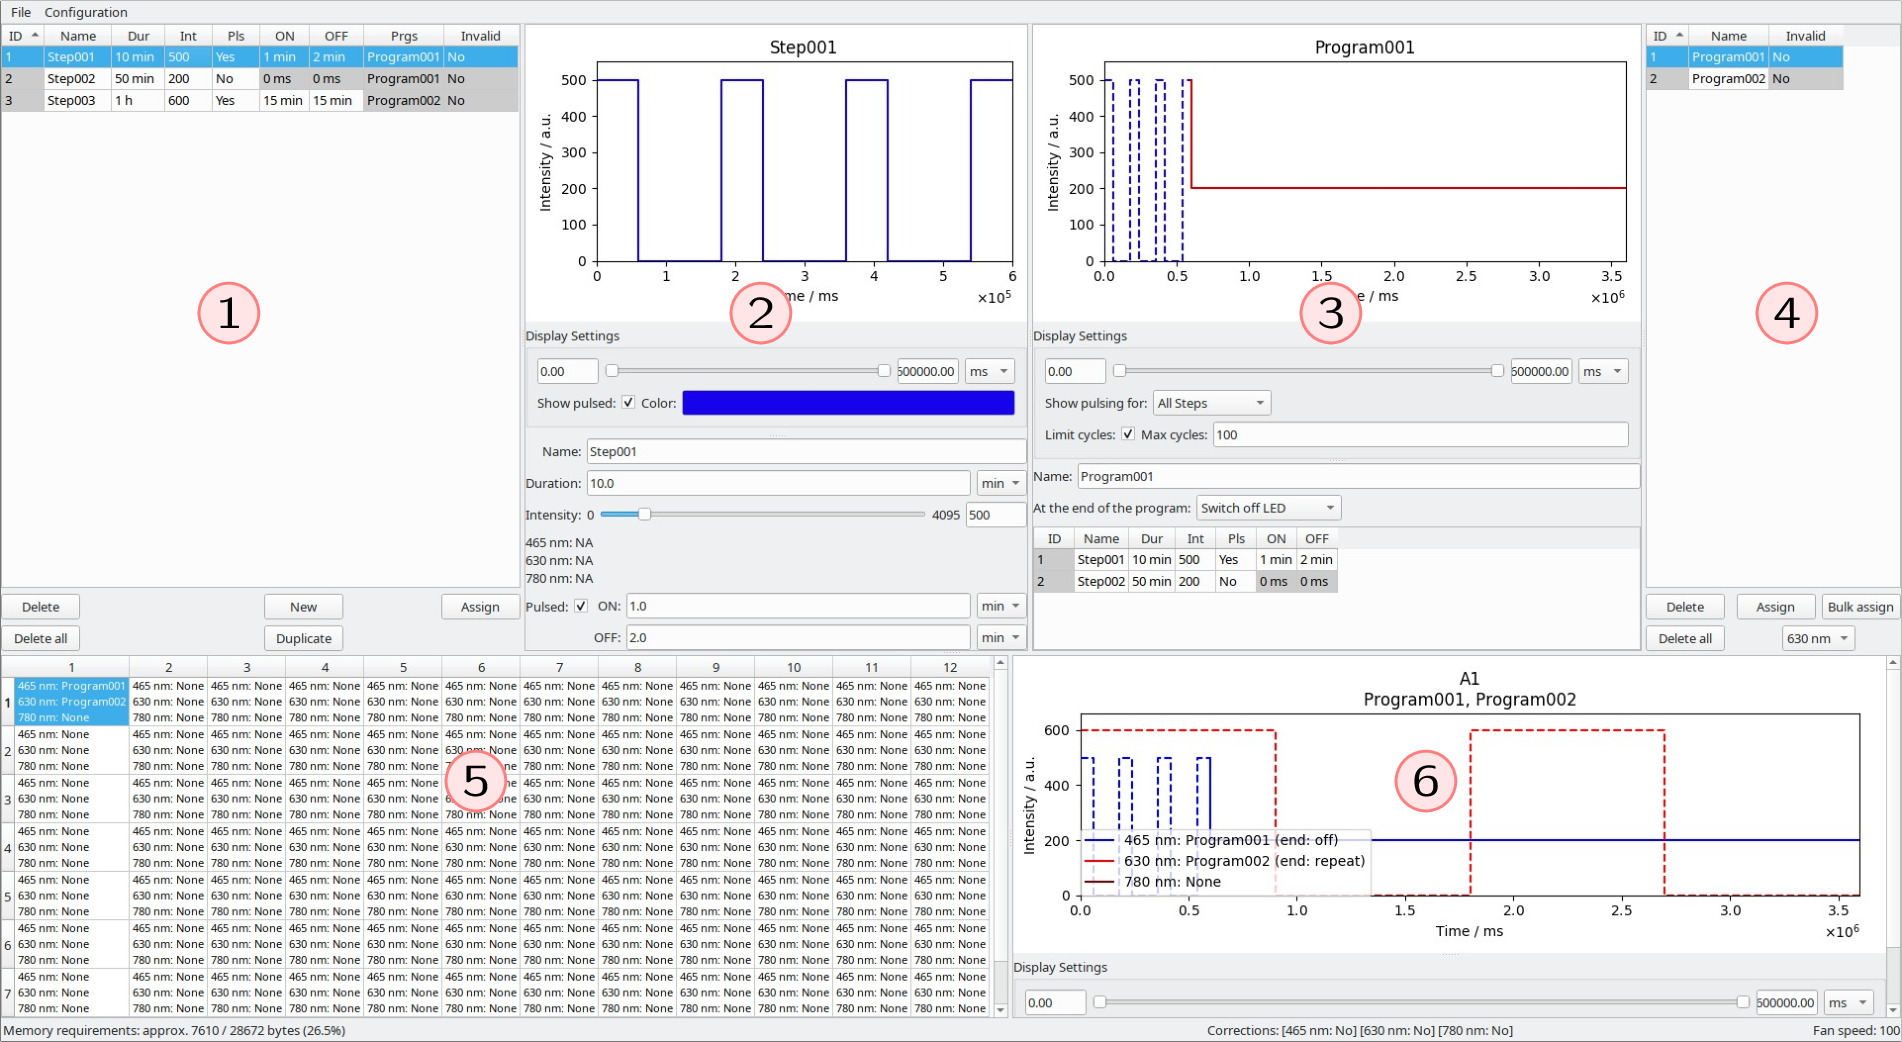
\includegraphics{images/annotated/overview.jpg}

\emph{The main application window.}

The application window is separated into a few distinct areas:

\begin{enumerate}
\def\labelenumi{\arabic{enumi}.}
\tightlist
\item
  Step List
\item
  Step Editor
\item
  Program Editor
\item
  Program List
\item
  Program Assignment
\item
  Well Viewer
\end{enumerate}

\hypertarget{step-list}{%
\subsubsection{Step List}\label{step-list}}

\begin{quote}
The Step list holds all defined Steps and displays information about
them in a tabular format. Steps are the building blocks of Programs.
Note that a Step is color-agnostic, i.e.~it does not know about the LED
it is controlling. Steps have a name and are defined by four parameters
(duration, intensity, pulse ON time, pulse OFF time). The time
parameters are limited to a resolution of 100 ms and can not be longer
than 4294967200 ms (approximately 49 days).
\end{quote}

\hypertarget{step-parameters}{%
\paragraph{Step Parameters}\label{step-parameters}}

\begin{itemize}
\item
  \emph{Name:}

  A name for the Step to easily find it in the Step list.
\item
  \emph{Duration:}

  The total duration of the Step.
\item
  \emph{Intensity:}

  Intensity of the Step, in arbitrary units from 0 (off) to 4095
  (maximum intensity). For pulsed Steps, this is the intensity during
  the ON phases. During the OFF phases, the intensity is 0. If desired,
  you may set conversion factors for each LED under \emph{Configuration
  \textgreater{} Configure Plate\ldots{}}, in order to display a
  conversion to physical units. \textbf{The converted values are only
  for illustration purposes and do not affect the output!}
\item
  \emph{Pulsed:}

  Indicates if the Step is a pulsed Step or a constant Step. Pulsed
  Steps always begin in the ON phase. If you need a Step to start with
  its OFF phase, you can add the Step to a Program and precede it with
  another Step of intensity 0 and the duration of the OFF phase.

  \begin{itemize}
  \item
    \emph{ON:} The duration of the ON phases.
  \item
    \emph{OFF:} The duration of the OFF phases.
  \end{itemize}
\end{itemize}

\hypertarget{table-columns}{%
\paragraph{Table columns}\label{table-columns}}

\begin{itemize}
\item
  \emph{ID, Name, Dur, Int, Pls, ON, OFF:}

  ID, name, duration, intensity, \emph{pulsed} status, pulse ON and
  pulse OFF time of the Step, respectively. The ID is assigned to the
  Step automatically and can not be changed.
\item
  \emph{Prgs:}

  The names of all Programs this Step is a part of.
\item
  \emph{Invalid:}

  If a Step is invalid, it cannot be exported to the Arduino. Invalid
  Steps are highlighted in red, and the cause of invalidity is displayed
  as a tooltip when you hover over them.
\end{itemize}

\hypertarget{buttons}{%
\paragraph{Buttons}\label{buttons}}

\begin{quote}
Below the Step list, common operations are immediately available.
\end{quote}

\begin{itemize}
\item
  \emph{Delete, Delete all:}

  Delete the selected Step, or all Steps at once.
\item
  \emph{New, Duplicate:}

  Create a new Step, or duplicate the selected Step.
\item
  \emph{Assign:}

  Add this Step to the active Program. The active Program is the one
  displayed in the Program Editor.
\end{itemize}

\hypertarget{context-menu}{%
\paragraph{Context Menu}\label{context-menu}}

\begin{quote}
Right clicking a Step in the list gives additional options.
\end{quote}

\begin{itemize}
\item
  \emph{Set Parameters for All Selected\ldots:}

  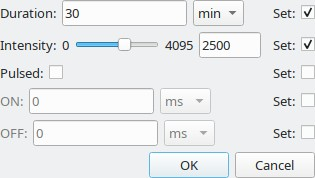
\includegraphics{images/setallparams.jpg}

  Opens a dialog in which all Step parameters can be defined. After
  clicking OK, all parameters for which \emph{Set} was selected are
  applied to all selected Steps.
\item
  \emph{Interpolate\ldots:}

  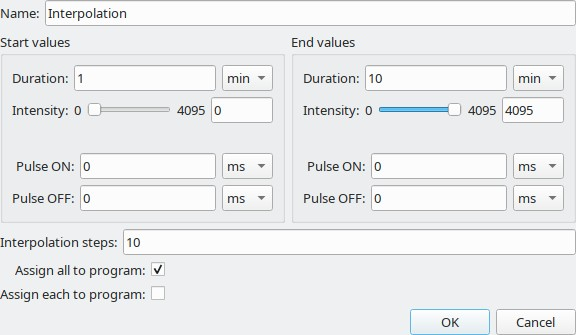
\includegraphics{images/interpolation_dialog.jpg}

  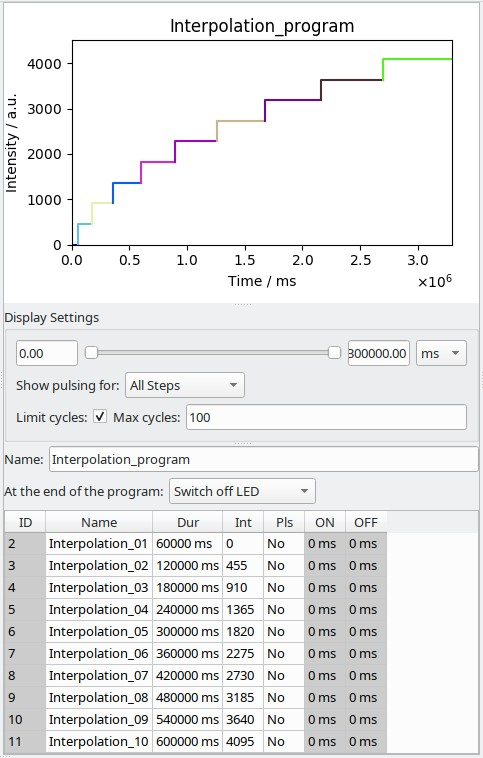
\includegraphics{images/interpolation_example.jpg}

  \emph{The interpolation dialog and the Steps (assembled in a Program)
  generated by these settings.}

  Opens a dialog in which new Steps can be created by linearly
  interpolating between boundaries for each parameter. The default
  values for the start and end values correspond to the parameters of
  the first and last selected Step, respectively. Interpolation can be
  used to quickly create a gradient illumination pattern, for instance
  with increasing or decreasing intensity over time.

  \begin{itemize}
  \tightlist
  \item
    \emph{Name:}
  \end{itemize}

  The prefix that will be added to the start of the names of generated
  Steps, followed by consecutive numbering. The name ``Interpolation''
  will generate Steps with names Interpolation\_1, Interpolation\_2,
  \ldots{}

  \begin{itemize}
  \tightlist
  \item
    \emph{Start values, End values:}
  \end{itemize}

  Set the parameter values to interpolate between here.

  \begin{itemize}
  \tightlist
  \item
    \emph{Interpolation steps}:
  \end{itemize}

  The number of Steps to generate.

  \begin{itemize}
  \tightlist
  \item
    \emph{Assign all to program:}
  \end{itemize}

  When this option is selected, a new Program is created which will
  contain all of the generated Steps in sequence.

  \begin{itemize}
  \tightlist
  \item
    \emph{Assign each to program:}
  \end{itemize}

  When this option is selected, a new Program is created \emph{for each
  individual Step}. This can be useful if you want to define gradients
  across multiple wells. Quickly assigning different programs to wells
  can be achieved by using the \emph{Bulk assign} operation, see section
  \emph{Program List} for details.
\item
  \emph{Assign Selected to Program\ldots:}

  Assign the selected Step(s) to a new or existing Program.
\end{itemize}

\begin{center}\rule{0.5\linewidth}{0.5pt}\end{center}

\hypertarget{step-editor}{%
\subsubsection{Step Editor}\label{step-editor}}

\begin{quote}
In the Step Editor, parameters are set for the Step which is currently
selected in the Step List.
\end{quote}

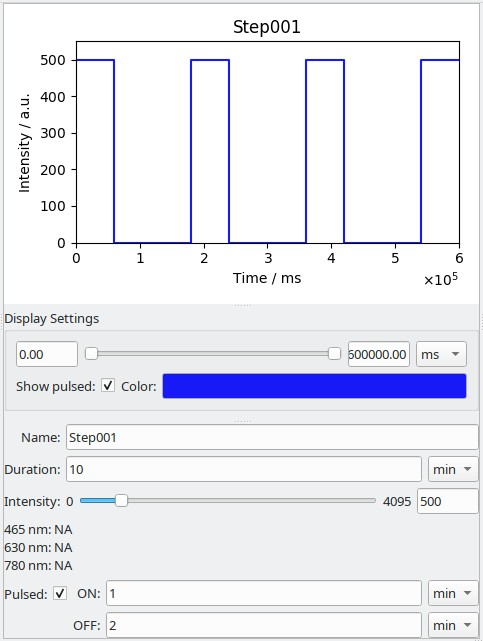
\includegraphics{images/stepeditor.jpg}

\emph{The Step Editor panel.}

\hypertarget{display-settings}{%
\paragraph{Display Settings}\label{display-settings}}

\begin{quote}
These settings do not influence the final Arduino output in any way and
only affect how the Step is displayed.
\end{quote}

\begin{itemize}
\item
  \emph{Range Slider:}

  The slider allows setting the X axis limits, which may be useful to
  verify short pulsing times for very long steps. In this case,
  individual pulses may no longer be clearly discernible.
\item
  \emph{Show pulsed:}

  When this option is turned off, the Step will not be displayed as
  pulsed. This can be useful for Steps which are very long, with very
  short pulsing times. This also affects how the Step is displayed in
  the Program Editor or the Well Viewer, when pulsing display is defined
  \emph{Per Step} there. Pulsed Steps which are shown unpulsed are
  plotted with the ON phase intensity - no averaging is performed.
\item
  \emph{Color:}

  The color used to plot the Step in the Step and Program Editors.
\end{itemize}

\hypertarget{step-parameters-1}{%
\paragraph{Step Parameters}\label{step-parameters-1}}

\protect\hyperlink{step-parameters}{See the explanation of Step
Parameters in the \emph{Step List} section.}

\begin{center}\rule{0.5\linewidth}{0.5pt}\end{center}

\hypertarget{program-editor}{%
\subsubsection{Program Editor}\label{program-editor}}

\begin{quote}
A Program is a collection of Steps which can be assigned to one or
multiple LEDs.
\end{quote}

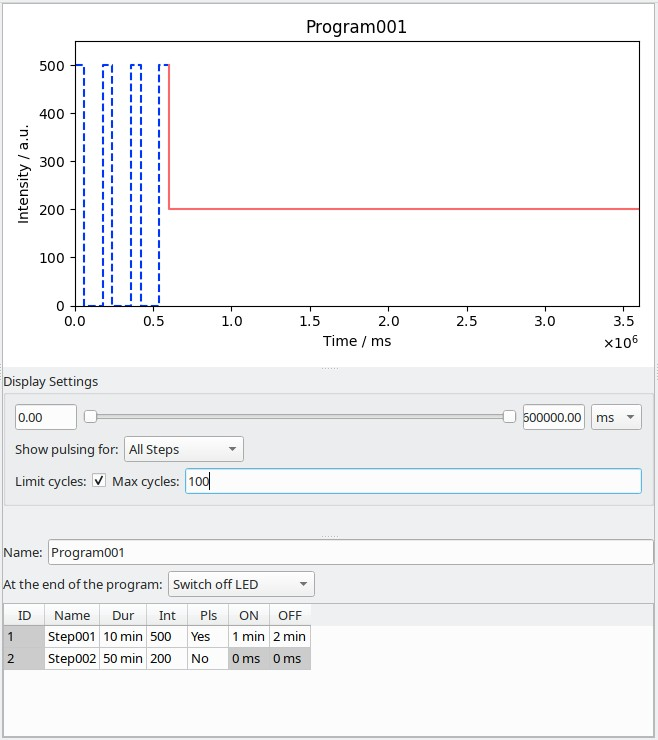
\includegraphics{images/programeditor.jpg}

\emph{The Program Editor panel.}

\hypertarget{display-settings-1}{%
\paragraph{Display Settings}\label{display-settings-1}}

\begin{quote}
These settings do not influence the final Arduino output in any way and
only affect how the Program is displayed.
\end{quote}

\begin{itemize}
\item
  \emph{Range Slider:}

  The slider allows setting the X axis limits, which may be useful to
  inspect short and long Steps in the same Program.
\item
  \emph{Show pulsing for:}

  Set this to determine how pulsing cycles are displayed. Depending on
  the duration of Steps in relation to their pulse on and off duration,
  the plot may appear visually cluttered, so disabling the pulse display
  may make it easier to discern. Note that even if pulses are not shown
  for a particular Step, it is plotted with a dashed line to indicate it
  is pulsed. Pulsed Steps which are shown unpulsed are plotted with the
  ON phase intensity - no averaging is performed.

  \begin{itemize}
  \item
    \emph{All Steps:}

    Pulsing is shown for all Steps in the Program.
  \item
    \emph{No Steps:}

    Pulsing is shown for no Steps in the Program.
  \item
    \emph{Define per Step:}

    Determine whether to show a Step pulsed by the \emph{Show pulsed}
    setting of the respective Step.
  \end{itemize}
\item
  \emph{Limit cycles, Mac cycles:}

  When this option is activated, the number of pulsing cycles that can
  be shown is capped at \emph{max cycles}. As long as all Steps in the
  active Program taken together do not undergo more pulsing cycles than
  the specified maximum, pulsing is plotted. When this value is
  exceeded, Steps are shown as constant to speed up the display. By
  default, this is set to 100. In this case, adding four Steps with 30
  pulsing cycles each would disable pulse plotting for the program.
\end{itemize}

\hypertarget{program-parameters}{%
\paragraph{Program Parameters}\label{program-parameters}}

\begin{quote}
A Program is assembled from a sequence of Steps and can be assigned to
one or multiple LEDs.
\end{quote}

\begin{itemize}
\item
  \emph{Name:}

  A name for the Program to easier find it in the Program list.
\item
  \emph{At the end of the program:}

  Defines what happens after all Steps in the Program were completed.

  \begin{itemize}
  \item
    \emph{Switch off LED:}

    After completion of all Steps, the LED to which this Program is
    assigned is turned off.
  \item
    \emph{Repeat the last step:}

    After completion of all Steps, the last Step in the Program is
    repeated indefinitely. While it is not possible to export Programs
    with a total Step duration of more than the maximum (approximately
    49 days), this limit may in principle be reached if a Step is set to
    repeat at the end of the Program. However, \textbf{this is not
    supported}!
  \end{itemize}

  The built-in LED on the Arduino Micro will blink when all Programs
  have completed all of their Steps at least once - it will also blink
  when a Program is set to repeat its last Step!
\item
  \emph{List of Steps in the Program:}

  Steps are executed in the order shown here. You can drag and drop
  Steps to re-arrange them. Right clicking on a Step allows the addition
  of a new Step to the Program, or removal of an existing Step from the
  Program.
\end{itemize}

\begin{center}\rule{0.5\linewidth}{0.5pt}\end{center}

\hypertarget{program-list}{%
\subsubsection{Program List}\label{program-list}}

\begin{quote}
The Program List holds all defined Programs and displays information
about them in a tabular format.
\end{quote}

\hypertarget{table-columns-1}{%
\paragraph{Table columns}\label{table-columns-1}}

\begin{itemize}
\item
  \emph{ID, Name:}

  ID and name of the Program, respectively.
\item
  \emph{Invalid:}

  If a Program is invalid, it cannot be exported to the Arduino. Invalid
  Programs are highlighted in red, and the cause of invalidity is
  displayed as a tooltip when you hover over them.
\end{itemize}

\hypertarget{buttons-1}{%
\paragraph{Buttons}\label{buttons-1}}

\begin{quote}
Below the Step list, common operations are immediately available:
\end{quote}

\begin{itemize}
\item
  \emph{Delete, Delete all:}

  Delete the selected Step, or all Steps at once.
\item
  \emph{LED Selector:}

  When clicking the \emph{Assign} or \emph{Bulk assign} buttons, the
  Program will be assigned to the selected wells. This menu specifies
  the LED to use for the assignment.
\item
  \emph{Assign:}

  Assign the selected Program to the selected Well and LED. To remove
  Programs from an LED, right click the respective well and choose
  \emph{Clear programs from selected wells}.
\item
  \emph{Bulk Assign:}

  This option allows assigning multiple Programs to multiple wells. It
  is only available when the same number of wells and Programs are
  selected. The selected Programs (in the order of selection) are
  assigned to the selected wells (likewise in the order of selection).

  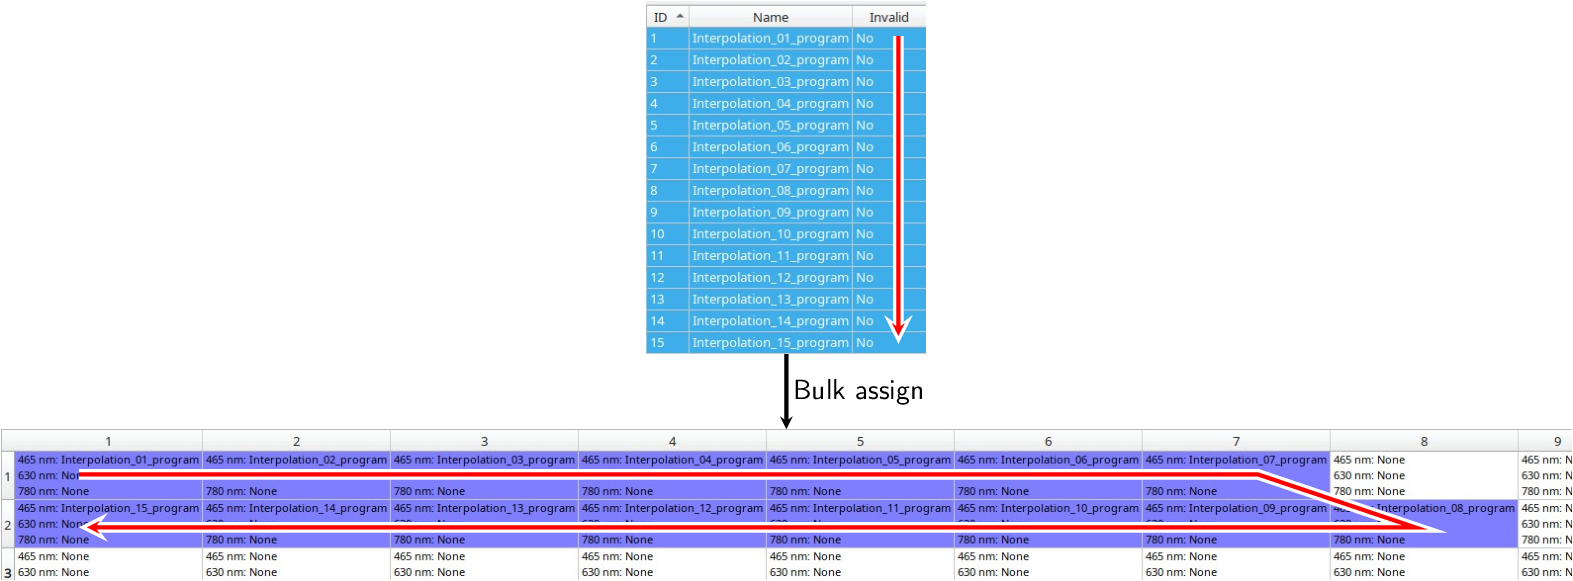
\includegraphics{images/annotated/bulk_assign.jpg}

  \emph{The result of a bulk assign operation. The arrows indicate the
  order of selection for Programs and wells, respectively. Note the
  names of the assigned Programs.}
\end{itemize}

\hypertarget{context-menu-1}{%
\paragraph{Context Menu}\label{context-menu-1}}

\begin{quote}
Right clicking a Program in the list gives additional options:
\end{quote}

\begin{itemize}
\item
  \emph{Create dark Step with program duration:}

  For each selected Program, creates a new Step with intensity 0 and
  duration equal to the sum of all Step durations in the respective
  Program. For instance, if a Program contains three 10 minute Steps,
  the dark Step would be 30 minutes long. This can be useful if Programs
  should be started in a staggered fashion between different wells: A
  dark Step is added to the start of the Program to achieve a delay.
\item
  \emph{Add program Steps to\ldots:}

  Adds the Steps of all selected Programs to another Program. This
  allows assembling Programs like building blocks. However, there is no
  link to the original Program after adding the Steps to another
  Program: If the source is modified after this operation, the changes
  will not be reflected in the destination.
\end{itemize}

\begin{center}\rule{0.5\linewidth}{0.5pt}\end{center}

\hypertarget{program-assignment}{%
\subsubsection{Program Assignment}\label{program-assignment}}

\begin{quote}
Here, the Programs which are assigned to the LEDs of a well are
displayed.
\end{quote}

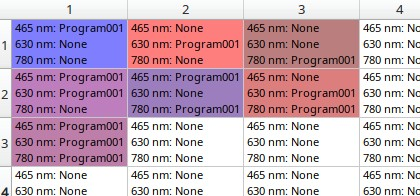
\includegraphics{images/well_colors.jpg}

The Program Assignment table is formatted like a multi-well plate: Table
rows correspond to plate rows, table columns correspond to plate
columns.

Each well can hold one Program per LED, but one Program can be assigned
to multiple LEDs. The names of all LEDs are shown in each cell, along
with the Program assigned to this LED. To facilitate visually
distinguishing the assignment patterns, the table cells are colored with
muted variations of the LED colors. If more than one LED is in use, a
mixed color is used. You can configure the names and colors of LEDs
under \emph{Configuration \textgreater{} Configure Plate\ldots{}}.

To remove Programs from an LED, right click the respective well and
choose \emph{Clear programs from selected wells}.

\begin{center}\rule{0.5\linewidth}{0.5pt}\end{center}

\hypertarget{well-viewer}{%
\subsubsection{Well Viewer}\label{well-viewer}}

\begin{quote}
The well viewer displays all Programs in a well at once.
\end{quote}

The colors that are used for the LEDs can be set under
\emph{Configuration \textgreater{} Configure Plate\ldots{}} and is
independent from the color set for the individual Steps.

\hypertarget{display-settings-2}{%
\paragraph{Display Settings}\label{display-settings-2}}

The display settings are the same as in the Program Editor, with one
addition:

\begin{itemize}
\item
  \emph{Show legend:}

  Toggles display of the legend. In the legend, the names of the
  Programs assigned to each LED are shown, as well as the action taken
  at the end of the Program (either \emph{off} or \emph{repeat}, as
  defined for the Program).
\end{itemize}

\begin{center}\rule{0.5\linewidth}{0.5pt}\end{center}

\hypertarget{exporting}{%
\subsubsection{Exporting}\label{exporting}}

After defining Steps, creating Programs and assigning them to LEDs, the
experimental setup is now ready to be exported to a code file that can
be uploaded to the Arduino. To do this, choose \emph{File \textgreater{}
Export}. You can either copy the code and paste it into the Arduino IDE
yourself, or choose \emph{Open in IDE} to launch the Arduino IDE.
Connect the Arduino controlling the optoPlate to your computer. In the
Arduino IDE, choose ``Arduino Micro'' under \emph{Tools \textgreater{}
Board}, and select the port to which the board is connected under
\emph{Tools \textgreater{} Port}. Then upload by choosing \emph{Sketch
\textgreater{} Upload}. For more help on uploading code to the Arduino,
see \href{https://www.arduino.cc/en/Guide/Environment\#uploading}{the
Arduino reference}.

Please note that LEDs may light up erratically if power is restored to
the Arduino Micro while it is connected to a computer via a Micro-USB
cable. To restore proper functionality, press the reset button on the
Arduino, or disconnect the Arduino from your computer and turn the power
off and back on again.

\begin{center}\rule{0.5\linewidth}{0.5pt}\end{center}

\hypertarget{the-configuration-menu}{%
\subsubsection{The Configuration Menu}\label{the-configuration-menu}}

\hypertarget{preferences}{%
\paragraph{Preferences}\label{preferences}}

In the preferences, you can set the path to the Arduino IDE, in order to
directly launch it from the Export window.

\hypertarget{configure-plate}{%
\paragraph{Configure Plate}\label{configure-plate}}

\begin{quote}
The plate configuration allows to set the grouping mode and the
characteristics of LED types.
\end{quote}

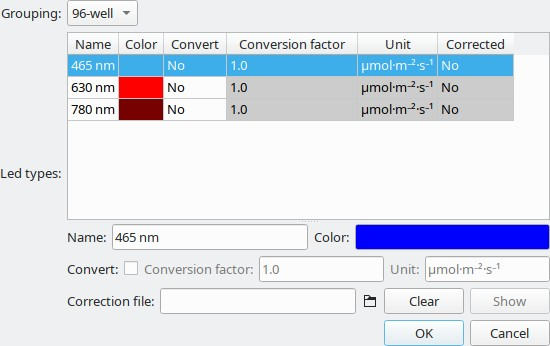
\includegraphics{images/plate_config.jpg}

\begin{itemize}
\item
  \emph{Grouping:}

  You can choose to assign Programs to each of the 96 wells of the
  optoPlate individually (\emph{96-well}), or you can select
  (\emph{24-well}) to perform assignment to groups of 4 wells, mimicking
  the layout of a 24-well plate. Note that changing the Grouping setting
  will reset all Program assignments.
\item
  \emph{LED types:}

  \begin{itemize}
  \item
    \emph{Name:}

    The name of the LED is used in the Program Assignment table and the
    Well Viewer and is only relevant for display purposes.
  \item
    \emph{Color:}

    The color assigned to an LED is used in the Program Assignment table
    and for the plots in the Well Viewer. It is only relevant for
    display purposes.
  \item
    \emph{Convert, Conversion factor, Unit:}

    If desired, a conversion factor can be entered to convert arbitrary
    units to physical units. This is shown in the Step Editor and can
    facilitate setting the necessary intensity for a Step. It is only
    relevant for display purposes, however, and has no effect on the
    exported intensities.
  \item
    \emph{Correction file:}

    You can specify the path to a .csv file which holds correction
    factors for LEDs. The file should be a comma-separated list of
    values, which can be exported from standard spreadsheet software. In
    both Microsoft Excel or LibreOffice Calc, .csv files can be saved by
    choosing \emph{File \textgreater{} Save As} and selecting .csv as
    the file type. The layout of the table must correspond to the layout
    of a multi-well plate (table rows to plate rows, table columns to
    plate columns).

    Each correction factor is a multiplication factor between 0.0 and
    1.0. When a Program runs on the optoPlate, each intensity is first
    multiplied by the correction factor before it is written to the LED.
    When a valid file was specified, the correction matrix can be shown
    with the \emph{Show} button. This feature can be used to reduce
    illumination differences between different wells, or to easily
    define intensity gradients over multiple wells of the plate, without
    having to define many Steps and Programs - simply assign the same
    Program to all LEDs and let the correction handle the creation of
    the gradient.

    Note that each LED type has its own correction factors and that they
    are not shared!

    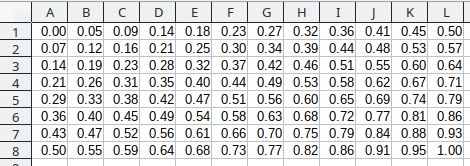
\includegraphics{images/corr_factors_sheet.jpg}

    \emph{Correction factors in a spreadsheet.}

    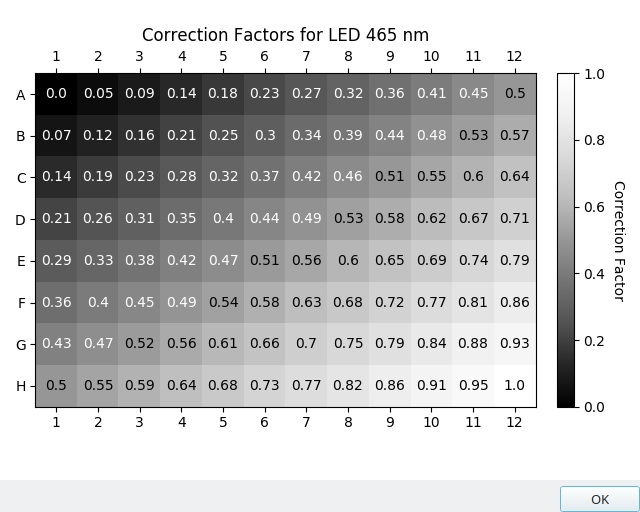
\includegraphics{images/corr_factors_show.jpg}

    \emph{Correction factors applied to an LED.}
  \end{itemize}
\end{itemize}

\hypertarget{set-fan-speed}{%
\paragraph{Set Fan Speed}\label{set-fan-speed}}

You can adjust the fan speed of the fan on the optoPlate from 0 (off) to
255 (maximum speed). The default value is 100. The fan speed needed to
provide sufficient cooling will depend on the heat generated by the
optoPlate during the protocol, which depends on the numbere of activated
LEDs and their intensities.

\begin{center}\rule{0.5\linewidth}{0.5pt}\end{center}

\hypertarget{the-status-bar}{%
\subsubsection{The Status Bar}\label{the-status-bar}}

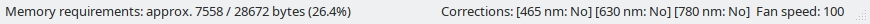
\includegraphics{images/statusbar.jpg}

\begin{itemize}
\item
  \emph{Memory requirements:}

  Displays an approximation of the storage space that will be required
  by the current configuration. The exact value varies between the
  platform and the version of the Arduino IDE, even for the same code.
  However, it can give you an indication of whether your current
  configuration is approaching the limits of the Arduino Micro.
\item
  \emph{Corrections:}

  Indicates which LED types have correction factors associated with
  them.
\item
  \emph{Fan speed:}

  Indicates the currently set fan speed. Adjust it under
  \emph{Configuration \textgreater{} Set Fan Speed \ldots{}}
\end{itemize}

\hypertarget{the-help-menu}{%
\subsubsection{The Help Menu}\label{the-help-menu}}

\hypertarget{about}{%
\paragraph{About}\label{about}}

Show information about optoConfig-96.

\hypertarget{examples}{%
\paragraph{Examples}\label{examples}}

You can pick from several example files made with optoConfig-96. These
mostly replicate the
\href{https://github.com/BugajLab/optoPlate-96/tree/master/2.\%20Code/1.\%20Arduino/2.\%20QCscripts}{quality
control scripts provided with the optoPlate-96}. Choosing one will open
it.

\hypertarget{user-guide}{%
\paragraph{User Guide}\label{user-guide}}

Opens the optoConfig-96 user guide in a browser.
